%% This is file `elsarticle-template-2-harv.tex',
%%
%% Copyright 2009 Elsevier Ltd
%%
%% This file is part of the 'Elsarticle Bundle'.
%% ---------------------------------------------
%%
%% It may be distributed under the conditions of the LaTeX Project Public
%% License, either version 1.2 of this license or (at your option) any
%% later version.  The latest version of this license is in
%%    http://www.latex-project.org/lppl.txt
%% and version 1.2 or later is part of all distributions of LaTeX
%% version 1999/12/01 or later.
%%
%% The list of all files belonging to the 'Elsarticle Bundle' is
%% given in the file `manifest.txt'.
%%
%% Template article for Elsevier's document class `elsarticle'
%% with harvard style bibliographic references
%%
%% $Id: elsarticle-template-2-harv.tex 155 2009-10-08 05:35:05Z rishi $
%% $URL: http://lenova.river-valley.com/svn/elsbst/trunk/elsarticle-template-2-harv.tex $
%%

%%\documentclass[preprint,authoryear,12pt]{elsarticle}

%% Use the option review to obtain double line spacing
%% \documentclass[authoryear,preprint,review,12pt]{elsarticle}

%% Use the options 1p,twocolumn; 3p; 3p,twocolumn; 5p; or 5p,twocolumn
%% for a journal layout:

%% Astronomy & Computing uses 5p
%% \documentclass[final,authoryear,5p,times]{elsarticle}
\documentclass[final,authoryear,5p,times,twocolumn]{elsarticle}

%% if you use PostScript figures in your article
%% use the graphics package for simple commands
%% \usepackage{graphics}
%% or use the graphicx package for more complicated commands
\usepackage{graphicx}
%% or use the epsfig package if you prefer to use the old commands
%% \usepackage{epsfig}

%% The amssymb package provides various useful mathematical symbols
\usepackage{amssymb}
%% The amsthm package provides extended theorem environments
%% \usepackage{amsthm}

\usepackage[pdftex,pdfpagemode={UseOutlines},bookmarks,bookmarksopen,colorlinks,linkcolor={blue},citecolor={green},urlcolor={red}]{hyperref}
\usepackage{hypernat}

%% Alternatives to hyperref for testing
%\usepackage{url}
%\newcommand{\htmladdnormallinkfoot}[2]{#1\footnote{\texttt{#2}}}
%\newcommand{\htmladdnormallink}[1]{\texttt{#1}}
%\newcommand{\href}[2]{\texttt{#2}}

%% The lineno packages adds line numbers. Start line numbering with
%% \begin{linenumbers}, end it with \end{linenumbers}. Or switch it on
%% for the whole article with \linenumbers after \end{frontmatter}.
%% \usepackage{lineno}

%% natbib.sty is loaded by default. However, natbib options can be
%% provided with \biboptions{...} command. Following options are
%% valid:

%%   round  -  round parentheses are used (default)
%%   square -  square brackets are used   [option]
%%   curly  -  curly braces are used      {option}
%%   angle  -  angle brackets are used    <option>
%%   semicolon  -  multiple citations separated by semi-colon (default)
%%   colon  - same as semicolon, an earlier confusion
%%   comma  -  separated by comma
%%   authoryear - selects author-year citations (default)
%%   numbers-  selects numerical citations
%%   super  -  numerical citations as superscripts
%%   sort   -  sorts multiple citations according to order in ref. list
%%   sort&compress   -  like sort, but also compresses numerical citations
%%   compress - compresses without sorting
%%   longnamesfirst  -  makes first citation full author list
%%
%% \biboptions{longnamesfirst,comma}

% \biboptions{}

\journal{Astronomy \& Computing}

%% Make single quotes look right in verbatim mode
\usepackage{upquote}

\usepackage{upgreek}

\usepackage{color}

\usepackage{listings}

\definecolor{mygreen}{rgb}{0,0.6,0}
\definecolor{mygray}{rgb}{0.5,0.5,0.5}
\definecolor{mymauve}{rgb}{0.58,0,0.82}

\lstset{ %
  backgroundcolor=\color{white},   % choose the background color
  basicstyle=\footnotesize\ttfamily,        % size of fonts used for the code
  breaklines=true,                 % automatic line breaking only at whitespace
  captionpos=b,                    % sets the caption-position to bottom
  commentstyle=\color{mygreen},    % comment style
  escapeinside={\%*}{*)},          % if you want to add LaTeX within your code
  keywordstyle=\color{blue},       % keyword style
  stringstyle=\color{mymauve},     % string literal style
}


% Aim to be consistent, and correct, about how we refer to sections
\newcommand*\secref[1]{Sect.~\ref{#1}}
\newcommand*\appref[1]{\ref{#1}}

\begin{document}

\begin{frontmatter}

%% Title, authors and addresses

%% use the tnoteref command within \title for footnotes;
%% use the tnotetext command for the associated footnote;
%% use the fnref command within \author or \address for footnotes;
%% use the fntext command for the associated footnote;
%% use the corref command within \author for corresponding author footnotes;
%% use the cortext command for the associated footnote;
%% use the ead command for the email address,
%% and the form \ead[url] for the home page:
%%
%% \title{Title\tnoteref{label1}}
%% \tnotetext[label1]{}
%% \author{Name\corref{cor1}\fnref{label2}}
%% \ead{email address}
%% \ead[url]{home page}
%% \fntext[label2]{}
%% \cortext[cor1]{}
%% \address{Address\fnref{label3}}
%% \fntext[label3]{}

\title{The Generalized Single-Dish Dataformat}

%% use optional labels to link authors explicitly to addresses:
%% \author[label1,label2]{<author name>}
%% \address[label1]{<address>}
%% \address[label2]{<address>}

\author[jac]{Tim Jenness\corref{cor1}\fnref{timj}}
\ead{t.jenness@jach.hawaii.edu}
\author[hp]{Jon Fairclough}
\author[nrao]{Richard~M.~Prestage}
\author[leiden,imapp]{Remo~P.~J.~Tilanus}

\cortext[cor1]{Corresponding author}
\fntext[timj]{Present address: Department of Astronomy, Cornell University, Ithaca,
  NY 14853, USA}

\address[jac]{Joint Astronomy Centre, 660 N.\ A`oh\=ok\=u Place, Hilo, HI
  96720, USA}
\address[hp]{HP Enterprise Services UK Ltd}
\address[nrao]{National Radio Astronomy Observatory, P.O.\ Box 2, Green Bank, WV~24944, USA}
\address[leiden]{Leiden Observatory, Leiden University, PO Box 9513, 2300 RA Leiden, The~Netherlands}
\address[imapp]{Department of Astrophysics,
     Institute for Mathematics, Astrophysics and Particle Physics,
     Radboud University Nijmegen, PO Box 9010, 6500 GL Nijmegen, The~Netherlands}

\begin{abstract}
%% Text of abstract

The Generalized Single-Dish Dataformat (GSDD) was developed in the
mid-1980s as a file format to support millimeter and submillimeter
instrumentation at NRAO, JCMT and IRAM. We discuss the implementation
of the file format, provide an overview of the GSDD requirements and
associated data model, cover its usage in the observatories and
provide a retrospective on the format.

\end{abstract}

\begin{keyword}
%% keywords here, in the form: keyword \sep keyword

%% MSC codes here, in the form: \MSC code \sep code
%% or \MSC[2008] code \sep code (2000 is the default)

data formats \sep submillimeter astronomy

\end{keyword}

\end{frontmatter}

% \linenumbers

%% Journal abbreviations
\newcommand{\mnras}{MNRAS}
\newcommand{\aap}{A\&A}
\newcommand{\aaps}{A\&AS}
\newcommand{\pasp}{PASP}
\newcommand{\apj}{ApJ}
\newcommand{\apjs}{ApJS}
\newcommand{\qjras}{QJRAS}
\newcommand{\an}{Astron.\ Nach.}
\newcommand{\ijimw}{Int.\ J.\ Infrared \& Millimeter Waves}
\newcommand{\procspie}{Proc.\ SPIE}
\newcommand{\aspconf}{ASP Conf. Ser.}

%% Applications

%% Misc

%% Links
\newcommand{\ascl}[1]{\href{http://www.ascl.net/#1}{ascl:#1}}

%% main text

\section{Introduction}

The Generalized Single Dish Data format (GSDD) was developed in the
1980s to solve the data processing and acquisition requirements of the
NRAO, IRAM and JCMT observatories. The format, agreed in 1986
\citep{mtdn85}, consisted of a data model for specifying millimeter
and submillimeter observations (continuum and heterodyne
instrumentation) and a specification of how the bytes would be
represented on disk. The goal was to drive interoperability between
the observatories to allow data taken at one telescope to be reduced
by software packages developed at another.

\section{Requirements}

As the sub-millimeter community began to develop in the 1980s it was
desirable to develop or adopt a single format that could be used
interchangeably. At the time two obvious options were available in the
astronomical community in the form of the Flexible Image Transport System
\citep[FITS;][]{1981A&AS...44..363W} and the Starlink Hierarchical
Data System \citep[HDS;][]{1982QJRAS..23..485D,2015HDS}.

A millimeter observation requires that many items of information are
stored that are multi-dimensional and time-varying requiring a storage
system that could support this and be self-describing.

FITS was discounted as the primary data format because of the large
amount of overhead required to format the header information when
writing files and the inability of the format to store more than one
data array or table in a file. FITS files at the time were not capable
of storing binary tables and ASCII tables were all that was possible
\citep{1988A&AS...73..365H}. It was also felt that the DEC Backup
Utility was more reliable for transport and archiving than using a
FITS tape format. It was felt that whilst the FITS community would
eventually support multiple data arrays and binary tables, it was not
possible to wait for that to happen.

HDS was discarded for I/O efficiency reasons and the inability for the
entire file to be mapped into memory in one operation. Given the
performance requirements for the JCMT data acquisition system it was
important that a file could be mapped using VMS system services as a
Global Section to allow other applications to get read access to the
contents of the file whilst it was being written. This led to the JCMT
implementation of the library being known as the Global Section
Datafile System \citep[GSD;][]{mtin33}\footnote{This naming of the
  library as GSD eventually led to JCMT users referring to the files
  as being of ``GSD format'' rather than ``GSDD format''.}.

These requirements led to a new format being devised and an associated
I/O library.

\section{File Format Design}

\begin{figure}
\begin{center}
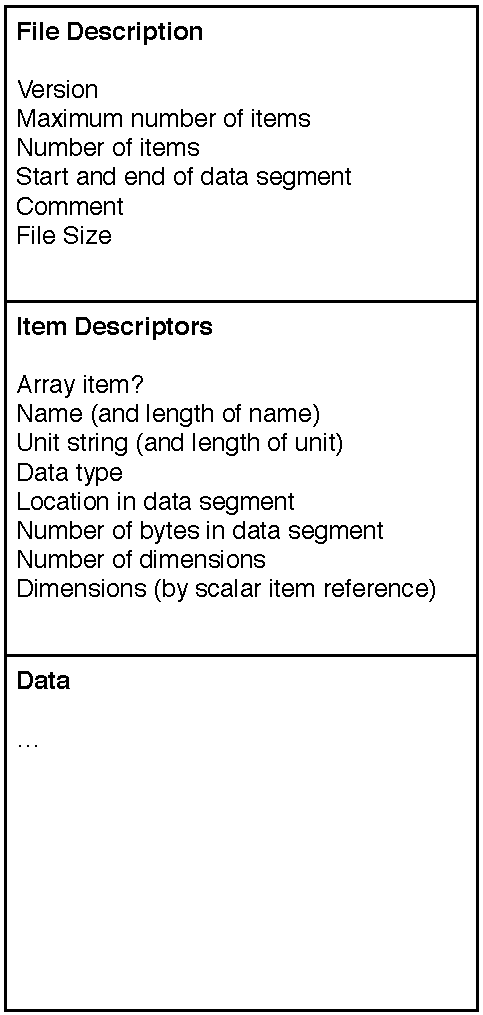
\includegraphics[width=0.5\columnwidth]{gsd-file-layout}
\end{center}
\caption{Layout of a JCMT GSDD data file. The file descriptor indicates
where the data starts and the number of items in the data. The item
descriptors describe each of those items and where they are located in
the data segment.}
\label{fig:jcmtgsd}
\end{figure}

The layout of a JCMT GSDD format file is show in
Fig.~\ref{fig:jcmtgsd} \citep[see also][]{mtdn84}. The file is split
into three segments: the file descriptor, the item descriptors and the
data itself. The file descriptor contains a general description of the
file indicating it's version, the number of items written and the
position of the data array. The item descriptors define each of the
items in terms of the label and units and the position in the data
array. For array items (GSDD supported up to 5 dimensions), the
identity of each dimension is specified in terms of the number of a
scalar item. This allows the label and unit to be associated with each
dimension of an array item in addition to the size of the
dimension. For example, the \texttt{C11PHA} array entry in a JCMT DAS
spectrum \citep{1986SPIE..598..134B} is dimensioned according to the
scalar items \texttt{C3NSV} and \texttt{C3PPC}, with a negative number
of dimensions indicating that an item is a scalar that defines an
array dimension.

The GSDD JCMT format supports the standard Fortran data
types of byte, word, logical, integer, real, double and character
strings. To simplify the format, character strings have a fixed size
of 16 characters, item names are fixed at 15 characters and unit
strings are fixed at 10 characters. The format supported the concept
of a ``null'' value by reserving the most negative value of each data
type for that purpose (using a single space as the null character value
and false as the null logical value). Additionally, the JCMT GSD
library supported data type conversion, allowing a user to request a
value in a different type to how it was stored natively in the file.

\section{Data Model}

To allow interoperability of data files between differing
observatories it was also important to develop a shared data model,
taking particular care to allow simple interchange of reduced spectra
between software packages. Reduced data has fewer instrument-specific
anomalies and was deemed to be the simplest first step, requiring
sufficient metadata to specify the coordinates of the spectrum on the
sky, the frequency scale and the calibrated
units of the spectrum.

\begin{table}
\caption{Model classes used by the GSDD model at JCMT.}
\label{tab:classes}
\begin{center}
\begin{tabular}{ll}
\hline
Class number & Meaning \\ \hline
1 & Identity Parameters\\
2 & Time Parameters\\
3 & Position Parameters\\
4 & Pointing Parameters \\
5 & Environment Parameters \\
6 & Mapping Parameters \\
7 & Velocity Parameters \\
8 & Engineering Parameters \\
9 & Data Parameters \\
10 & Receiver Parameters\\
11 & Phase Control Table \\
12 & Phase Value Table \\
13 & Phase Timing Table \\
14 & Data Value Table \\
15 & Pointing History \\
55 & Inclinometry \\
\hline
\end{tabular}
\end{center}
\end{table}

When designing the model related items were grouped into numbered
classes and the parameter name was prefixed by that class number. For
example \texttt{C13DAT} referred to the spectrum and bolometer data,
\texttt{C1SNO} the scan number, and \texttt{C7VR} the source radial velocity.

At the JCMT these ``NRAO'' names were mapped to local equivalents in
the acquisition computers (for example \texttt{C12RF}, the rest
frequency, mapped to \texttt{FE\_NUREST} in the acquisition system and
was equivalent to the \texttt{RESTFREQ} FITS keyword). A full list of
the equivalences can be found in \citet{SUN229}.

{\color{red}
Some of these class names now seem strange given that
\texttt{C13DAT} is the data of interest but is not in Class 14, and
the time, \texttt{C3DAT} is not in Class 2\ldots Is there an NRAO
data model document anywhere?
}



\section{Format Usage}

\subsection{James Clerk Maxwell Telescope}

The JCMT took data in the GSDD format for all instruments (heterodyne
and continuum) from the telescope commissioning (circa 1986) to the
delivery of SCUBA in 1996 \citep{1999MNRAS.303..659H}. The GSDD format
continued to be used for heterodyne instruments until the delivery of
the new ACSIS correlator in 2006 \citep{2009MNRAS.399.1026B}. SCUBA
and the new instruments wrote data in the Starlink extensible
\emph{N}-dimensional Data Format \citep[NDF;][]{2015NDF}, although
SCUBA's data model did not exactly match that used for ACSIS and
SCUBA-2 \citep{2013MNRAS.430.2513H} data. The GSD data access library
was a VAX-specific library \citep{1986QJRAS..27..675.,mtdn84} written
in Fortran and making extensive use of VAX system calls. When
the last instrument moved off of the VAX/VMS data acquisitions computers
the format could no longer be used and was retired.

The GSDD data files were archived at the Canadian Astronomy Data
Centre and approximately 440\,000 GSDD format files are in the
archive, totalling approximately 30\,GB. In order to access these data
files on a Unix system a new read-only version of the GSD library was
written in C \citep{SUN229} and integrated into the standard data
reduction tools SPECX \citep[][\ascl{1310.008}]{SPECX}, COADD
\citep[][\ascl{1411.020}]{COADD}  and JCMTDR
\citep[][\ascl{1406.019}]{SUN132}.  The GSDD format is relatively
simple and the main complication in the new C (and later pure Java)
implementations was the conversion of VAX floating point format to
IEEE format.

There is currently a plan at the Joint Astronomy Centre to convert the
heterodyne files to the modern ACSIS format such that they can be
reduced using the standard JCMT data reduction pipelines
\citep{2015ACSISDR}. The standard SMURF data reduction application
(\ascl{1310.007}\nocite{2013ascl.soft10007J}) contains the ability to
read GSD files and migrate them to the modern format \citep{SUN259}.

The GSDD files from the earlier continuum instruments, such as UKT14 \citep{1990MNRAS.243..126D}, will
remain in the archive although they will not be visible in the JCMT
Science Archive \citep{2015Economou}.

\subsection{National Radio Astronomy Observatory}

\ldots

{\color{red}

  UNIPOPS used SDD format which is like GSD but used IEEE floating
  point natively rather than VAX floating point \citep{UNIPOPS}.

  SDD format in that UNIPOPS document seems slightly different to the
  JCMT implementation. It also evolved by changing the integer data
  type.

  Was the NRAO format the same on the VAX? Was it used for acquisition
  or just data processing?
}

\section{Retrospective}

{\color{red}

What happened at NRAO? Did IRAM take any notice of GSDD? They looked
like they were part of the 1986 discussion.

There was a meeting at Green Bank in late
1989\footnote{\url{http://fits.gsfc.nasa.gov/dishfits/dishfits.8910}}
to discuss how the millimeter community could migrate to a
single-dish format based on FITS.

Looks like this helped drive the adoption of binary tables in FITS
\citep{1995A&AS..113..159C} and ultimately the SDFITS standard
\citep{2000ASPC..216..243G}. Collaboration between JCMT and NRAO
dissolved as JCMT continued to use and develop ``GSD'' but NRAO
migrated to SDFITS.

Was GSD a successful format? Yes, in terms of its longevity at JCMT.

When the JCMT control system was built, computing performance was a
major concern. For this reason HDS and FITS, which were not designed
for real-time operation and were deemed too slow. The JCMT software
team had experience of in-memory data management - those who had
worked at MRAO had used shared memory for data capture and those from
SERC who had worked with the ADAM MON system knew how to manage a
shared database. The GSD software library took ideas from the MON
system to provide a suite of routines for memory management that
provided the required performance. It was a forerunner of the
in-memory databases we see today.

Are there any lessons on the standardization process that we can
report on? Why did it fail? What could have been done differently?

GSD was documented and stable. The UK had Starlink to publish the
software and data files to the UK community. Access to that network
from other countries, such as the US, was problematic, and hindered
the spread of the software and prevented take up. Fears of lack of
support also drive people to create their own in-house
solutions. Today, the internet and the culture of open-source
development make that much less likely and a good idea has a better
chance of surviving and growing.

}

It was solely used as a data acquisition format at JCMT, with there
being one application on the VAX to enable the editing of contents if
there was a need to fix some metadata. Data reduction applications
never wrote data out in GSDD format, as evidenced by there not being
any requirement to have the ability to write new files in the
applications ported to Unix.

{\color{red}
A perl interface to the Unix C GSD library to allow preview of spectra
for remote observers when doing flexible scheduling
\citep{1997ASPC..125..401J}.
}




\section{Conclusions}

{\color{red}
Maybe will be covered in previous section.
}

The GSDD format was used for twenty years at the JCMT\ldots

\section*{Acknowledgments}

The James Clerk Maxwell Telescope has historically been operated by
the Joint Astronomy Centre on behalf of the Science and Technology
Facilities Council of the United Kingdom, the National Research
Council of Canada and the Netherlands Organisation for Scientific
Research.

The source code for the JCMT GSD library (C, Perl wrapper, and Java)
is available from
\htmladdnormallinkfoot{Github}{https://github.com/Starlink/starlink}
and distributed under the Gnu General Public Licence.

%% References
%%
%% Following citation commands can be used in the body text:
%%
%%  \citet{key}  ==>>  Jones et al. (1990)
%%  \citep{key}  ==>>  (Jones et al., 1990)
%%
%% Multiple citations as normal:
%% \citep{key1,key2}         ==>> (Jones et al., 1990; Smith, 1989)
%%                            or  (Jones et al., 1990, 1991)
%%                            or  (Jones et al., 1990a,b)
%% \cite{key} is the equivalent of \citet{key} in author-year mode
%%
%% Full author lists may be forced with \citet* or \citep*, e.g.
%%   \citep*{key}            ==>> (Jones, Baker, and Williams, 1990)
%%
%% Optional notes as:
%%   \citep[chap. 2]{key}    ==>> (Jones et al., 1990, chap. 2)
%%   \citep[e.g.,][]{key}    ==>> (e.g., Jones et al., 1990)
%%   \citep[see][pg. 34]{key}==>> (see Jones et al., 1990, pg. 34)
%%  (Note: in standard LaTeX, only one note is allowed, after the ref.
%%   Here, one note is like the standard, two make pre- and post-notes.)
%%
%%   \citealt{key}          ==>> Jones et al. 1990
%%   \citealt*{key}         ==>> Jones, Baker, and Williams 1990
%%   \citealp{key}          ==>> Jones et al., 1990
%%   \citealp*{key}         ==>> Jones, Baker, and Williams, 1990
%%
%% Additional citation possibilities
%%   \citeauthor{key}       ==>> Jones et al.
%%   \citeauthor*{key}      ==>> Jones, Baker, and Williams
%%   \citeyear{key}         ==>> 1990
%%   \citeyearpar{key}      ==>> (1990)
%%   \citetext{priv. comm.} ==>> (priv. comm.)
%%   \citenum{key}          ==>> 11 [non-superscripted]
%% Note: full author lists depends on whether the bib style supports them;
%%       if not, the abbreviated list is printed even when full requested.
%%
%% For names like della Robbia at the start of a sentence, use
%%   \Citet{dRob98}         ==>> Della Robbia (1998)
%%   \Citep{dRob98}         ==>> (Della Robbia, 1998)
%%   \Citeauthor{dRob98}    ==>> Della Robbia


%% References with bibTeX database:

\bibliographystyle{model2-names-astronomy}
\bibliography{acgsd}

%% Authors are advised to submit their bibtex database files. They are
%% requested to list a bibtex style file in the manuscript if they do
%% not want to use model2-names.bst.

%% References without bibTeX database:

% \begin{thebibliography}{00}

%% \bibitem must have one of the following forms:
%%   \bibitem[Jones et al.(1990)]{key}...
%%   \bibitem[Jones et al.(1990)Jones, Baker, and Williams]{key}...
%%   \bibitem[Jones et al., 1990]{key}...
%%   \bibitem[\protect\citeauthoryear{Jones, Baker, and Williams}{Jones
%%       et al.}{1990}]{key}...
%%   \bibitem[\protect\citeauthoryear{Jones et al.}{1990}]{key}...
%%   \bibitem[\protect\astroncite{Jones et al.}{1990}]{key}...
%%   \bibitem[\protect\citename{Jones et al., }1990]{key}...
%%   \harvarditem[Jones et al.]{Jones, Baker, and Williams}{1990}{key}...
%%

% \bibitem[ ()]{}

% \end{thebibliography}

\end{document}

%%
%% End of file `elsarticle-template-2-harv.tex'.
